% Created by tikzDevice version 0.6.2-92-0ad2792 on 2013-04-07 17:57:35
% !TEX encoding = UTF-8 Unicode
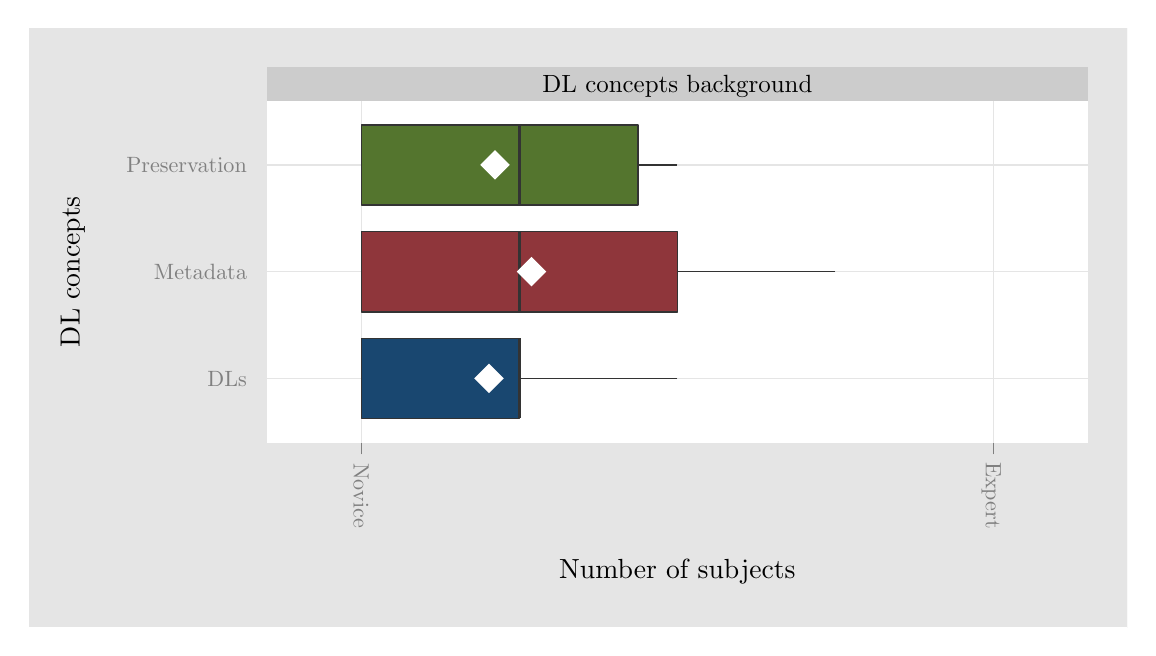
\begin{tikzpicture}[x=1pt,y=1pt]
\definecolor[named]{fillColor}{rgb}{1.00,1.00,1.00}
\path[use as bounding box,fill=fillColor,fill opacity=0.00] (0,0) rectangle (397.48,216.81);
\begin{scope}
\path[clip] (  0.00,  0.00) rectangle (397.48,216.81);
\definecolor[named]{drawColor}{rgb}{1.00,1.00,1.00}
\definecolor[named]{fillColor}{rgb}{0.90,0.90,0.90}

\path[draw=drawColor,line width= 0.6pt,line join=round,line cap=round,fill=fillColor] (  0.00,  0.00) rectangle (397.48,216.81);
\end{scope}
\begin{scope}
\path[clip] ( 86.31, 66.91) rectangle (383.26,190.36);
\definecolor[named]{fillColor}{rgb}{1.00,1.00,1.00}

\path[fill=fillColor] ( 86.31, 66.91) rectangle (383.26,190.36);
\definecolor[named]{drawColor}{rgb}{0.90,0.90,0.90}

\path[draw=drawColor,line width= 0.6pt,line join=round] ( 86.31, 90.06) --
	(383.26, 90.06);

\path[draw=drawColor,line width= 0.6pt,line join=round] ( 86.31,128.64) --
	(383.26,128.64);

\path[draw=drawColor,line width= 0.6pt,line join=round] ( 86.31,167.22) --
	(383.26,167.22);

\path[draw=drawColor,line width= 0.6pt,line join=round] (120.57, 66.91) --
	(120.57,190.36);

\path[draw=drawColor,line width= 0.6pt,line join=round] (349.00, 66.91) --
	(349.00,190.36);
\definecolor[named]{drawColor}{rgb}{0.20,0.20,0.20}
\definecolor[named]{fillColor}{rgb}{0.20,0.20,0.20}

\path[draw=drawColor,line width= 0.6pt,line join=round,fill=fillColor] (177.68, 90.06) -- (234.78, 90.06);

\path[draw=drawColor,line width= 0.6pt,line join=round,fill=fillColor] (120.57, 90.06) -- (120.57, 90.06);
\definecolor[named]{fillColor}{rgb}{0.10,0.28,0.44}

\path[draw=drawColor,line width= 0.6pt,line join=round,line cap=round,fill=fillColor] (177.68, 75.59) --
	(120.57, 75.59) --
	(120.57,104.53) --
	(177.68,104.53) --
	(177.68, 75.59) --
	cycle;
\definecolor[named]{fillColor}{rgb}{0.20,0.20,0.20}

\path[draw=drawColor,line width= 1.1pt,line join=round,fill=fillColor] (177.68, 75.59) -- (177.68,104.53);

\path[draw=drawColor,line width= 0.6pt,line join=round,fill=fillColor] (234.78,128.64) -- (291.89,128.64);

\path[draw=drawColor,line width= 0.6pt,line join=round,fill=fillColor] (120.57,128.64) -- (120.57,128.64);
\definecolor[named]{fillColor}{rgb}{0.56,0.21,0.23}

\path[draw=drawColor,line width= 0.6pt,line join=round,line cap=round,fill=fillColor] (234.78,114.17) --
	(120.57,114.17) --
	(120.57,143.10) --
	(234.78,143.10) --
	(234.78,114.17) --
	cycle;
\definecolor[named]{fillColor}{rgb}{0.20,0.20,0.20}

\path[draw=drawColor,line width= 1.1pt,line join=round,fill=fillColor] (177.68,114.17) -- (177.68,143.10);

\path[draw=drawColor,line width= 0.6pt,line join=round,fill=fillColor] (220.51,167.22) -- (234.78,167.22);

\path[draw=drawColor,line width= 0.6pt,line join=round,fill=fillColor] (120.57,167.22) -- (120.57,167.22);
\definecolor[named]{fillColor}{rgb}{0.33,0.46,0.18}

\path[draw=drawColor,line width= 0.6pt,line join=round,line cap=round,fill=fillColor] (220.51,152.75) --
	(120.57,152.75) --
	(120.57,181.68) --
	(220.51,181.68) --
	(220.51,152.75) --
	cycle;
\definecolor[named]{fillColor}{rgb}{0.20,0.20,0.20}

\path[draw=drawColor,line width= 1.1pt,line join=round,fill=fillColor] (177.68,152.75) -- (177.68,181.68);
\definecolor[named]{fillColor}{rgb}{1.00,1.00,1.00}

\path[fill=fillColor] (161.36, 90.06) --
	(166.70, 95.39) --
	(172.03, 90.06) --
	(166.70, 84.72) --
	cycle;

\path[fill=fillColor] (176.74,128.64) --
	(182.07,133.97) --
	(187.41,128.64) --
	(182.07,123.30) --
	cycle;

\path[fill=fillColor] (163.56,167.22) --
	(168.89,172.55) --
	(174.23,167.22) --
	(168.89,161.88) --
	cycle;
\end{scope}
\begin{scope}
\path[clip] (  0.00,  0.00) rectangle (397.48,216.81);
\definecolor[named]{fillColor}{rgb}{0.80,0.80,0.80}

\path[fill=fillColor] ( 86.31,190.36) rectangle (383.26,202.58);
\definecolor[named]{drawColor}{rgb}{0.00,0.00,0.00}

\node[text=drawColor,anchor=base,inner sep=0pt, outer sep=0pt, scale=  0.90] at (234.78,193.37) {DL concepts background};
\end{scope}
\begin{scope}
\path[clip] (  0.00,  0.00) rectangle (397.48,216.81);
\definecolor[named]{drawColor}{rgb}{0.50,0.50,0.50}

\node[text=drawColor,anchor=base east,inner sep=0pt, outer sep=0pt, scale=  0.80] at ( 79.19, 87.30) {DLs};

\node[text=drawColor,anchor=base east,inner sep=0pt, outer sep=0pt, scale=  0.80] at ( 79.19,125.88) {Metadata};

\node[text=drawColor,anchor=base east,inner sep=0pt, outer sep=0pt, scale=  0.80] at ( 79.19,164.46) {Preservation};
\end{scope}
\begin{scope}
\path[clip] (  0.00,  0.00) rectangle (397.48,216.81);
\definecolor[named]{drawColor}{rgb}{0.50,0.50,0.50}

\path[draw=drawColor,line width= 0.6pt,line join=round] (120.57, 62.64) --
	(120.57, 66.91);

\path[draw=drawColor,line width= 0.6pt,line join=round] (349.00, 62.64) --
	(349.00, 66.91);
\end{scope}
\begin{scope}
\path[clip] (  0.00,  0.00) rectangle (397.48,216.81);
\definecolor[named]{drawColor}{rgb}{0.50,0.50,0.50}

\node[text=drawColor,rotate=270.00,anchor=base,inner sep=0pt, outer sep=0pt, scale=  0.80] at (117.82, 47.74) {Novice};

\node[text=drawColor,rotate=270.00,anchor=base,inner sep=0pt, outer sep=0pt, scale=  0.80] at (346.24, 47.74) {Expert};
\end{scope}
\begin{scope}
\path[clip] (  0.00,  0.00) rectangle (397.48,216.81);
\definecolor[named]{drawColor}{rgb}{0.00,0.00,0.00}

\node[text=drawColor,anchor=base,inner sep=0pt, outer sep=0pt, scale=  1.00] at (234.78, 17.94) {Number of subjects};
\end{scope}
\begin{scope}
\path[clip] (  0.00,  0.00) rectangle (397.48,216.81);
\definecolor[named]{drawColor}{rgb}{0.00,0.00,0.00}

\node[text=drawColor,rotate= 90.00,anchor=base,inner sep=0pt, outer sep=0pt, scale=  1.00] at ( 18.80,128.64) {DL concepts};
\end{scope}
\end{tikzpicture}
